\section{Generalities}
\subsection{Power}
All primary displays use electrical power from the secondary AC bus.
The displays are turned on by the yellow top-left button on the TI
(\cockpitref{fig:front-panel}{item:TI}).
In addition, displays are turned on at takeoff when RPM exceeds 90\%.

The HUD requires 40 seconds of preheating after AC power is available, before turning on.

\section{Head Up Display (HUD)}
\subsection{Overview}
\begin{figure}[!ht]
  \centering
  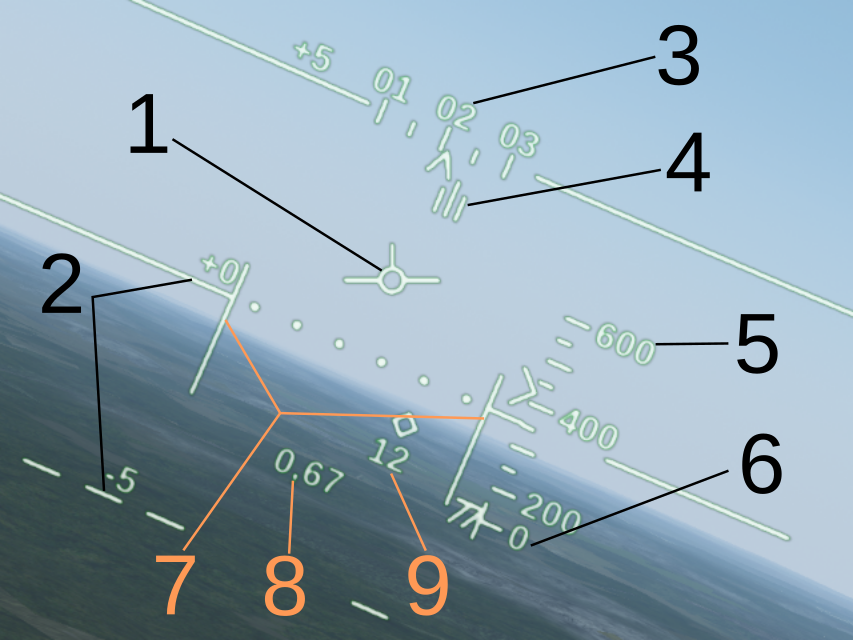
\includegraphics[width=0.7\textwidth]{images/displays/ja-hud-general.png}

  \begin{multicols}{2}
    \begin{enumerate}[nosep]
      \item \label{item:fpv} Flight path vector
      \item \label{item:horizon} Artificial horizon and pitch lines
      \item \label{item:heading} Heading scale
      \item \label{item:dest} Destination bearing
      \item \label{item:altitude} Altitude scale
      \item \label{item:rhm} Radar altimeter index and reference
      \item \label{item:altbars} Altitude bars
      \item \label{item:speed} Airspeed / Mach indicator
      \item \label{item:distance} Distance indicator
    \end{enumerate}
  \end{multicols}

  \caption{HUD overview}
  \label{fig:hud}
\end{figure}

\paragraph{Artificial Horizon (\cockpitref{fig:hud}{item:horizon})}
The artificial horizon and pitch scale provide an attitude reference.
The pitch scale consists of a line every 5 degrees.
Lines above the horizon are solid, lines below the horizon are dashed.
The artificial horizon itself is distinguished by six center dots.
Only the three pitch lines closest to the flight path vector are displayed.

\paragraph{Flight Path Vector (\cockpitref{fig:hud}{item:fpv})}
The FPV marker indicates the aircraft path direction relative to the ground.
Most of the HUD is centered around the FPV marker.

\paragraph{Heading Scale (\cockpitref{fig:hud}{item:heading})}
The heading scale is located above the FPV.
The fixed wedge index indicates aircraft track angle.
The second index consisting of 3 vertical lines
(\cockpitref{fig:hud}{item:dest}) indicates bearing to the next waypoint.

\paragraph{Altitude Scale (\cockpitref{fig:hud}{item:altitude})}
The altitude scale is located right of the FPV.
The fixed wedge index indicates aircraft altitude.
At low altitude the scale zooms in,
allowing to read the altitude more precisely for low level flight.

When the radar altimeter is active and in range,
the altitude 0 mark is displayed just below the altitude scale
(\cockpitref{fig:hud}{item:rhm}).
The radar altitude index, consisting of two wedges, can be read against this mark.
This can be used to set the altimeter QFE in flight.

\paragraph{Altitude Bars (\cockpitref{fig:hud}{item:altbars})}
The two altitude bars indicate the reference altitude
(also called commanded altitude) relative to the current altitude.

The top of the altitude bars represents commanded altitude,
while the artificial horizon represents current altitude.
If the top of the bars is on the horizon, the aircraft is at the commanded altitude.
If the top of the bars is above (resp.\ below) the horizon,
the aircraft is below (resp.\ above) the commanded altitude.

When the FPV is within 1\textdegree{} of the horizon,
the altitude scale index is fixed on the horizon.
Under these conditions, the top of the altitude bars
can be read on the altitude scale to obtain the commanded altitude.

Altitude bars are only displayed below 1000m.
When autopilot altitude hold is active, boxes are displayed together with
(below 1000m) or instead of (above 1000m) the altitude bars.

\subparagraph{Reference Altitude}
\label{sec:ref-alt}
The reference altitude displayed by the altitude bars is set as follows.
\begin{itemize}[noitemsep]
  \item During takeoff, the altitude bars are fixed over the horizon.
    After leaving takeoff mode, reference altitude is set to 500m.
  \item During flight, the reference button (keybinding \keys{\shift+R})
    sets the reference altitude to the current altitude.
  \item If autopilot altitude hold mode is active,
    the reference altitude is the autopilot altitude.
  \item When entering landing mode, reference altitude is set to 500m.
    It can still be modified with the reference button or by engaging autopilot altitude hold.
\end{itemize}

\paragraph{Airspeed / Mach Indicator (\cockpitref{fig:hud}{item:speed})}
Digital airspeed is displayed below the FPV,
with a minimum of 75km/h and a precision of 5km/h
(40kts and 1kts respectively in imperial units mode).
Above M 0.5, airspeed is replaced by a Mach indicator.

\paragraph{Distance Indicator (\cockpitref{fig:hud}{item:distance})}
Displays digital distance to the next waypoint.

\paragraph{Radar Altitude}
When radar altitude is less than 100m, it is displayed digitally
in the lower left part of the HUD, with the format e.g.\ `R 45'.
It is hidden for 30s after exiting takeoff mode, and in landing mode.

\paragraph{Ground Collision Warning}
Ground collision warning is displayed on the HUD as
a flashing arrow over the FPV, pointing in the pull-up direction.

\paragraph{Text Indications}
To the lower left of the FPV, plain text indications
can be shown in the following priority order:
\begin{enumerate}
  \item Altimeter setting warning `QFE' (flashing).
    At takeoff, indicates that the altimeter is incorrectly set.
    In flight, indicates that the altimeter should be switched to/from STD mode
    (assumes transition altitude 1500m).
  \item In landing mode, `TILS' indication when receiving ILS signal.
    (flashing if glideslope is not available or not in range).
  \item Selected weapon type (at the earliest 30s after leaving takeoff mode).
\end{enumerate}


\subsection{Takeoff Mode}
\begin{figure}[!ht]
  \centering
  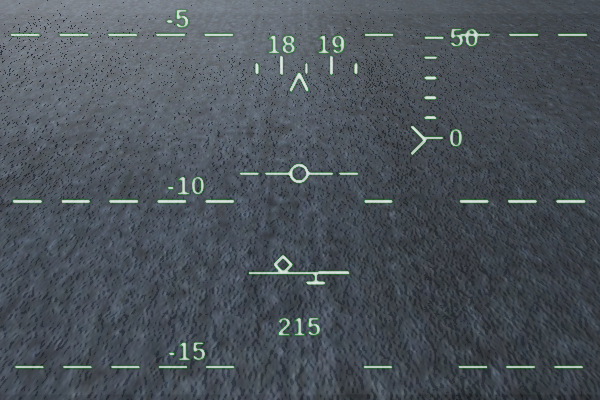
\includegraphics[width=0.5\textwidth]{images/displays/ja-hud-takeoff.png}
  \caption{HUD during takeoff}
  \label{fig:hud-takeoff}
\end{figure}

Takeoff mode is enabled when the nose gear is compressed.

During takeoff, the FPV is fixed vertically 10\textdegree{}
below the aircraft forward axis, and its symbol changes.
Horizontally, the FPV functions as in navigation mode,
and will e.g.\ move due to sidewind after rotation.

The distance line is displayed below the FPV, and represents airspeed.
The diamond upper index indicates aircraft speed,
and the inverted-T bottom marker indicates recommended rotation speed.
When the rotation angle reaches 5\textdegree{}, the distance line is hidden.

Takeoff mode stops once the airspeed exceeds M 0.35,
when the climb angle is at least 3\textdegree{},
or at landing gear retraction.

\subsection{Landing Mode}
\begin{figure}[!ht]
  \centering
  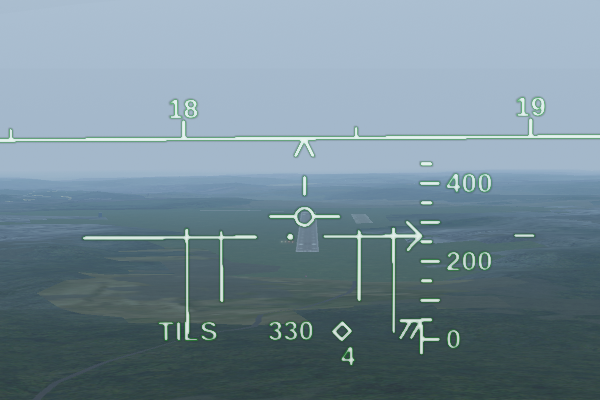
\includegraphics[width=0.5\textwidth]{images/displays/ja-hud-landing.png}
  \caption{HUD during final}
  \label{fig:hud-landing}
\end{figure}

In landing mode, the HUD changes when starting the final.
The -5\textdegree{} pitch line is removed,
and a glideslope line is added 2.86\textdegree{} below the horizon
(corresponding to a slope of 5\%).
Altitude scale, digital airspeed, and distance indicator are positioned around the glideslope line.
Heading scale is positioned over the horizon, and changes to a 1:1 scale.
Altitude bars are hidden.

If the climb or dive angle exceeds $\pm 7.5\degree$,
the default presentation of the pitch scale, digital airspeed, and distance indicator is restored,
while the heading and altitude scales are hidden.

\paragraph{Speed / AoA Indicator}
In landing mode, the vertical fin (`tail') of the flight path vector symbol
moves vertically to indicate deviation from the target speed or angle of attack.

The speed is correct when the bottom of the tail is on the FPV circle
(default position in navigation mode).
If the tail is higher than the circle, the aircraft speed is too high.
If the tail is lower (inside the circle), the aircraft speed is too low.

While the landing gear is up, the target speed is 550km/h.
Once the landing gear is down and locked, the target angle of attack is
computed based on aircraft weight, with a maximum of 12\textdegree{}
(15.5\textdegree{} if the button \cockpitref{fig:front-panel}{item:autothrottle-lights} is pressed and lit).

When the landing gear is down, the fin will blink if the angle of attack is critically high.

\paragraph{ILS Guidance}
If ILS guidance is used, the reference point on the glideslope line
indicates the heading to follow to align with the localizer.
Four vertical bars on the glideslope line indicate ILS glideslope deviation:
if the top of the bars is above, resp.\ below the glideslope line,
the aircraft is below, resp.\ above the ILS glideslope.

If ILS is not used (optical landing mode),
the reference point is aligned with the FPV, and the vertical bars are hidden.

\paragraph{Touchdown}
Below 35m, the HUD switches to optical landing display (ILS indications disappear).
Below 15m radar altitude, the HUD switches to flare mode.
The glideslope line moves up to indicate the descent angle
which gives a vertical speed of 2.8m/s, the maximum for touchdown.
If radar altitude is unavailable, transition to flare mode occurs at 35m.

Once the nose gear is compressed, the HUD switches to takeoff mode.

\subsection{Tactical Information}
Some tactical information is displayed on the HUD when a weapon is selected,
when a radar contact is tracked, and while in aiming mode.
%See \cref{chap:weapons} for details.


\section{Target Display (MI)}
The MI (\cockpitref{fig:front-panel}{item:MI}) is the JA 37 main radar display.

\subsection{Overview}
\label{sec:mi-overview}
The following indication lights and buttons are located around the MI display.
\begin{figure}[!ht]
  \centering
  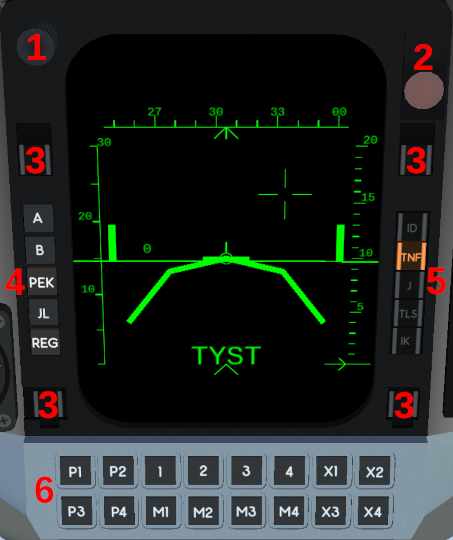
\includegraphics[width=0.5\textwidth]{images/displays/MI-overview.png}

  \begin{multicols}{2}
    \begin{enumerate}[nosep]
      \item \label{item:brightness} Brightness setting knob
      \item \label{item:gpw} Ground proximity warning light
      \item \label{item:mlw} Missile warning lights
      \item \label{item:buttons} Left side buttons
      \item \label{item:lights} Right side indication lights
      \item \label{item:bot-buttons} Bottom buttons
    \end{enumerate}
  \end{multicols}

  \caption{MI indication lights and buttons}
  \label{fig:mi}
\end{figure}

\paragraph{Left side buttons (\cockpitref{fig:mi}{item:buttons})}
\begin{description}[nosep]
  \item[A/B] TI display map zoom out/in
  \item[PEK/JL] Fighter control / fighter link controls (not implemented)
  \item[REG] Recorder (not implemented)
\end{description}

\paragraph{Right side lights (\cockpitref{fig:mi}{item:lights})}
\begin{description}[nosep]
  \item[ID/J] Radar modes (not implemented)
  \item[TNF] Inertia navigation alignment indicator
  \item[TLS] TILS signal indicator
  \item[IK] Identification transponder (not implemented)
\end{description}

\paragraph{Bottom buttons (\cockpitref{fig:mi}{item:bot-buttons})}
Pressing button P3 displays a help text on the MI (\cockpitref{fig:mi-screen}{item:text-help}).

\begin{tabular}{lll}
  button & help text & function \\
  \hline
  P1 & D       & Radar interference mode (not implemented) \\
  2  & SVY/SDV & Toggle TI sideview display \\
  M2 & VMI/RWR & Toggle TI radar warning display \\
  M4 & TNF/INN & Reset interial navigation \\
  X1 & BIT     & Start RB 99 built in test \\
  X2 & LNK     & Toggle RB 99 datalink \\
  X3 & HÄN/EVN & Register manual event
\end{tabular}

Other buttons have no functionality in the real aircraft.

\subsection{Display Overview}
\begin{figure}[!ht]
  \centering
  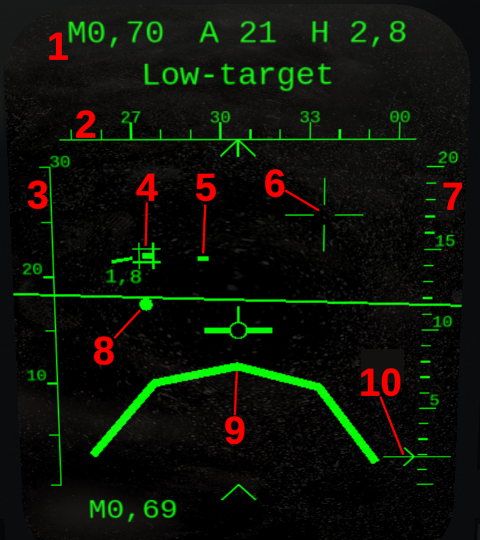
\includegraphics[width=0.48\textwidth]{images/displays/MI-overview1.png}
  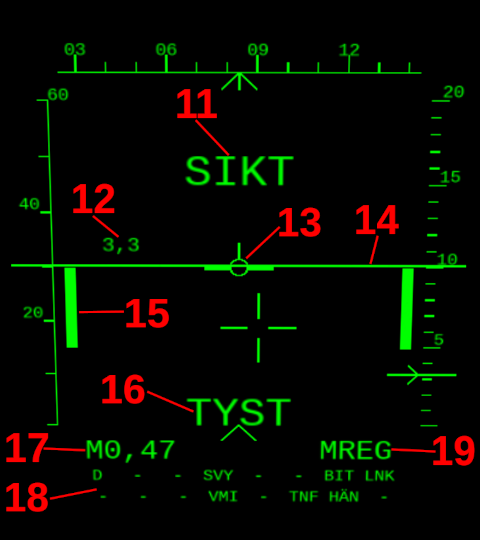
\includegraphics[width=0.48\textwidth]{images/displays/MI-overview2.png}

  \begin{multicols}{2}
    \begin{enumerate}[nosep]
      \item \label{item:tgt-info} Selected contact information
      \item \label{item:heading} Heading scale
      \item \label{item:distance} Distance scale
      \item \label{item:selected} Selected radar contact
      \item \label{item:contact} Other radar contact
      \item \label{item:cursor} Cursor
      \item \label{item:altitude} Altitude scale
      \item \label{item:azimuth} Selected contact azimuth / elevation
      \item \label{item:ground} Ground proximity indicator
      \item \label{item:alt-index} Altitude index
      \item \label{item:text-sikt} Text: HUD aiming mode
      \item \label{item:dig-alt} Digital altitude
      \item \label{item:fpv} Flight path marker
      \item \label{item:horizon} Artificial horizon
      \item \label{item:alt-bars} Altitude reference bars
      \item \label{item:text-tyst} Text: radar silent
      \item \label{item:text-mach} Bottom left text (here: Mach indicator)
      \item \label{item:text-help} Bottom text: (here: buttons help)
      \item \label{item:text-mreg} Bottom right text (here: manual event)
    \end{enumerate}
  \end{multicols}

  \caption{MI display overview}
  \label{fig:mi-screen}
\end{figure}

\subsection{Flight Indications}
\paragraph{%
  Artificial Horizon (\cockpitref{fig:mi-screen}{item:horizon})
  and Flight Path Marker (\cockpitref{fig:mi-screen}{item:fpv})
}
The flight path marker is fixed, and serves as a reference for the artificial horizon.
The artificial horizon line rotates to indicate roll,
and deviates from the flight path marker to indicate flight path angle.
Deviation is proportional to the sine of the flight path angle.

\paragraph{Altitude Indications}
Digital altitude (\cockpitref{fig:mi-screen}{item:dig-alt}) is displayed above the artificial horizon.
A marker (\cockpitref{fig:mi-screen}{item:alt-index}) indicates altitude
on the altitude scale (\cockpitref{fig:mi-screen}{item:altitude}), on the right side.

Altitude bars (\cockpitref{fig:mi-screen}{item:alt-bars}) are read against the artificial horizon,
and indicate reference altitude relative to the current altitude.
The top of the altitude bars represents reference altitude,
while the artificial horizon represents current altitude.
If the top of the bars is on the horizon, the aircraft is at the commanded altitude.
If the top of the bars is above (resp.\ below) the horizon,
the aircraft is below (resp.\ above) the commanded altitude.
Altitude bars are displayed below 1000m, or when autopilot altitude hold is active.

Ground height measured by the radar altimeter is displayed by a chevron index on each altitude bar,
when the radar altitude is less than 600m.

\paragraph{Ground Proximity Warning}
The distance between the ground symbol (\cockpitref{fig:mi-screen}{item:ground})
and the flight path marker (\cockpitref{fig:mi-screen}{item:fpv})
indicates margin from a ground proximity warning.
When the ground symbol touches the flight path marker, a ground proximity warning occurs.
On the MI, it is indicated by a flashing arrow on the flight path marker pointing in the pull-up direction,
as well as the flashing ground proximity warning light (\cockpitref{fig:mi}{item:gpw}).

\subsection{Text Messages}
The following text indications can be displayed on the MI.

\paragraph{SIKT / AIM (\cockpitref{fig:mi-screen}{item:text-sikt})}
Indicates that the HUD is in aiming mode.

\paragraph{TYST / SILENT (\cockpitref{fig:mi-screen}{item:text-tyst})}
Indicates that the radar is off.

\paragraph{Bottom left (\cockpitref{fig:mi-screen}{item:text-mach})}
The following indications can be displayed, by order of priority:
\begin{enumerate}[nosep]
  \item Altimeter setting warning `QFE' (flashing). Same conditions as on the HUD.
  \item Selected weapon type, if any.
  \item Mach number, at M>0.4.
\end{enumerate}

\paragraph{Bottom right (\cockpitref{fig:mi-screen}{item:text-mreg})}
The following indications can be displayed, by order of priority:
\begin{enumerate}[nosep]
  \item MREG, indicating a manually registered event (button X3 below the MI \cockpitref{fig:mi}{item:bot-buttons})
  \item FÖ / FAIL, indicating an aircraft failure. Goes off when consulting the TI failure page.
\end{enumerate}

\paragraph{Bottom (\cockpitref{fig:mi-screen}{item:text-help})}
The following indications can be displayed, by order of priority:
\begin{enumerate}[nosep]
  \item Memo for the MI lower buttons (\cockpitref{fig:mi}{item:bot-buttons}),
    when pressing button `P3' (cf.~\cref{sec:mi-overview}).
  \item RB 99 datalink estimated time to target and chance of hit,
    enabled with button X2.
\end{enumerate}

\subsection{Radar Display}
The radar display, at the center of the MI screen, is a B-scope,
i.e.\ the x-axis represents bearing, read against the heading scale (\cockpitref{fig:mi-screen}{item:heading}),
and the y-axis represents distance, read against the distance scale (\cockpitref{fig:mi-screen}{item:distance}).
The heading scale has a range of $\pm 60\degree$ around the aircraft heading.
The distance scale range is the same as the radar range (modified with \keys{[}/\keys{]}).
Radar echoes are displayed as small bars (\cockpitref{fig:mi-screen}{item:contact}).

\paragraph{Selected Contact}
The cursor (\cockpitref{fig:mi-screen}{item:cursor}) can be moved across the radar display.
Selecting a radar contact allows to track it. See \cref{sec:cursor} for controls.
When a radar contact is tracked, it is displayed on the HUD and TI,
and additional information on that contact is displayed on the MI.
On the radar display, the selected echo is surrounded by a \# sign (\cockpitref{fig:mi-screen}{item:selected}),
and a line starting from the selected echo indicates its heading and true speed.
The contact speed (Mach), distance, and altitude are displayed
at the top of the MI (\cockpitref{fig:mi-screen}{item:tgt-info}).
In FlightGear, the contact callsign and aircraft type are also displayed just below
(\keys{I} to toggle between callsign and type).
A dot (\cockpitref{fig:mi-screen}{item:azimuth}) indicates the contact azimuth and elevation,
read relative to the flight path marker.

\paragraph{IFF}
When a contact is selected, an IFF interogation is automatically performed.
Furthermore, manual IFF queries can be done by moving the cursor over a radar echo and pressing \keys{\ctrl+F}.
In either case, if the radar contact is friendly, a cross will be displayed over it.
For the selected contact, this cross replaces the usual \# sign.
In case of a manual IFF query, a small square indicates that the echo did not give a friendly return.
These symbols are summarized in \cref{fig:mi-iff}.
See also \cref{sec:iff} regarding the IFF system.

\begin{figure}
  \begin{tikzpicture}
    \draw node at (0,0) {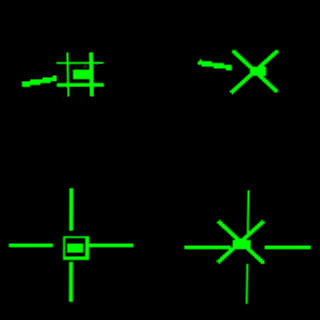
\includegraphics[width=0.3\textwidth]{images/displays/MI-iff.png}};
    \draw node at (-5,1) {Selected radar contact};
    \draw node at (-5,-1) {Manual IFF query};
    \draw node at (-1.2,2.5) {Hostile};
    \draw node at (1.2,2.5) {Friendly};
  \end{tikzpicture}

  \caption{MI IFF symbols.}
  \label{fig:mi-iff}
\end{figure}

\subsection{Missile Launch Zone Indication}
If a missile is selected, armed, and locked on the tracked radar contact,
several cues are displayed at the center of the MI,
indicating target range relative to missile performance.
The cues appear in the following order, as the target distance diminishes:
\begin{enumerate}[nosep]
  \item At the maximum firing range, a circle arc with the top-left quadrant missing appears.
  \item As the target range decreases, this circle grows until reaching optimistic launch range.
  \item When the target is in the no-escape-zone, the top-left arc appears, completing the circle.
  \item When the target is inside the minimum firing range, the circle is replaced by a large cross.
\end{enumerate}
